\section{Dataset Description}

The dataset for this project was obtained from a Kaggle repository titled \textit{Dangerous Heartbeat Dataset (DHD)} \cite{Dangerous-Heartbeat-Dataset-DHD}, 
which in turn sources its data from the PASCAL Classifying Heart Sounds Challenge 2011 (CHSC2011) \cite{pascal-chsc-2011}. 
This dataset comprises audio recordings of heartbeats, categorized into different types of heart sounds.
Specifically, the dataset consists of 5 types of recordings: Normal Heart Sounds, Murmur Sounds, Extra Heart Sounds, Extrasystole Sounds, and Artifacts.
Data has been gathered from the general public via the iStethoscope Pro iPhone app and from a clinic trial in hospitals using the digital stethoscope DigiScope.

\subsection{Data Exploration}


\begin{figure}[H]
    \centering
    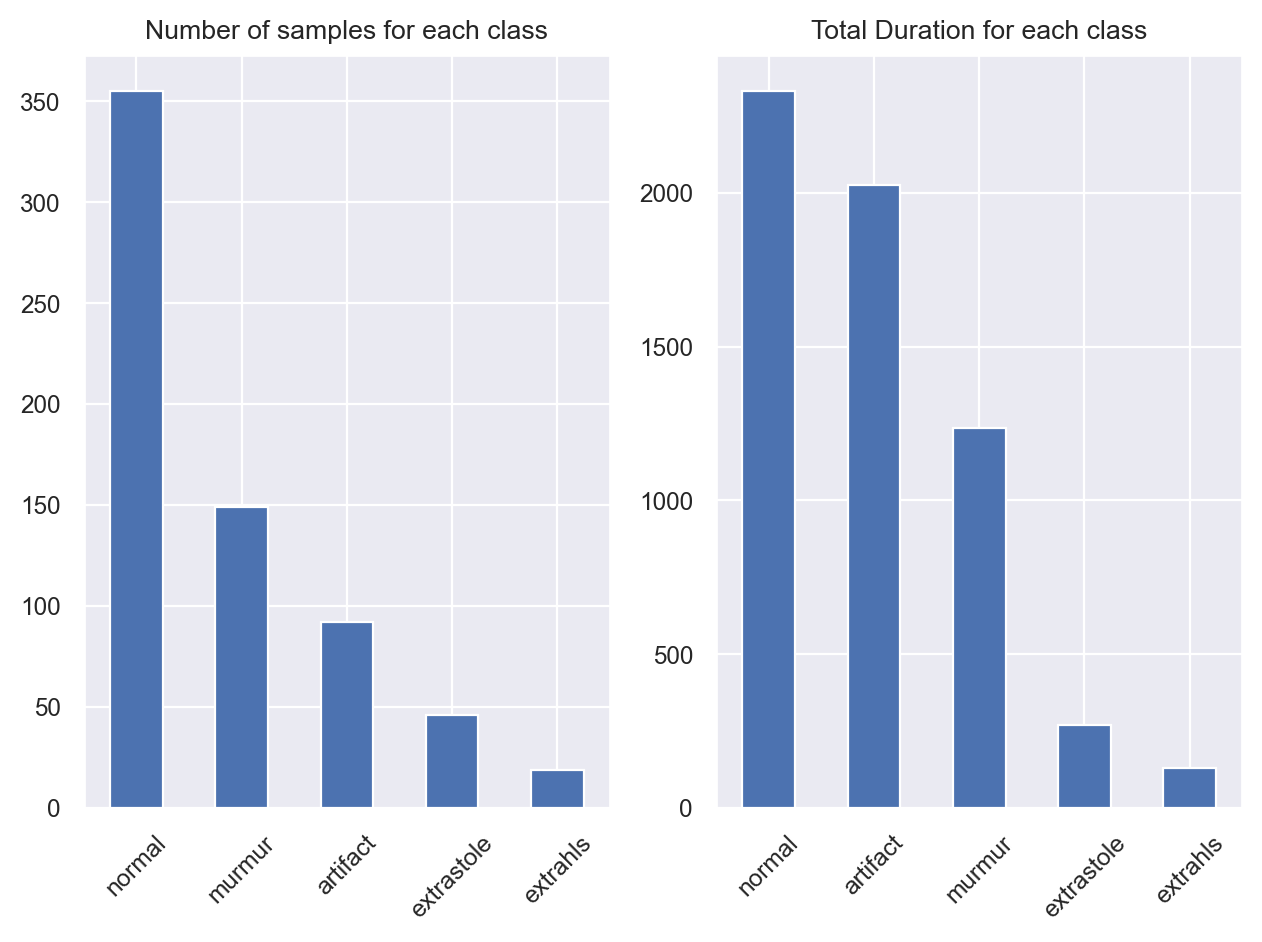
\includegraphics[width=1\columnwidth]{./images/DataExp_num_durations.png}
    \caption{Number of samples per duration.}
    \label{fig:DataExp_num_durations}
\end{figure}

\begin{figure}[H]
    \centering
    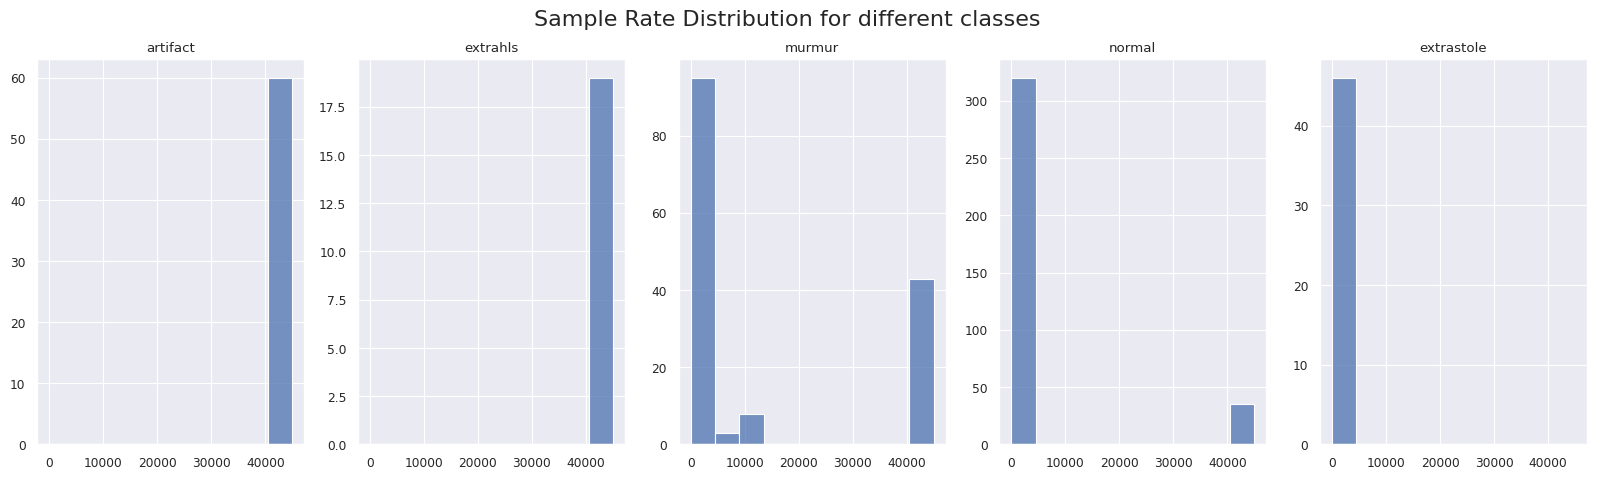
\includegraphics[width=1\columnwidth]{./images/DataExp_sr_distribution.png}
    \caption{Distribution of sampling rates.}
    \label{fig:DataExp_sr_distribution}
\end{figure}

\subsection{Data Preprocessing}

\begin{figure}[H]
	\centering
	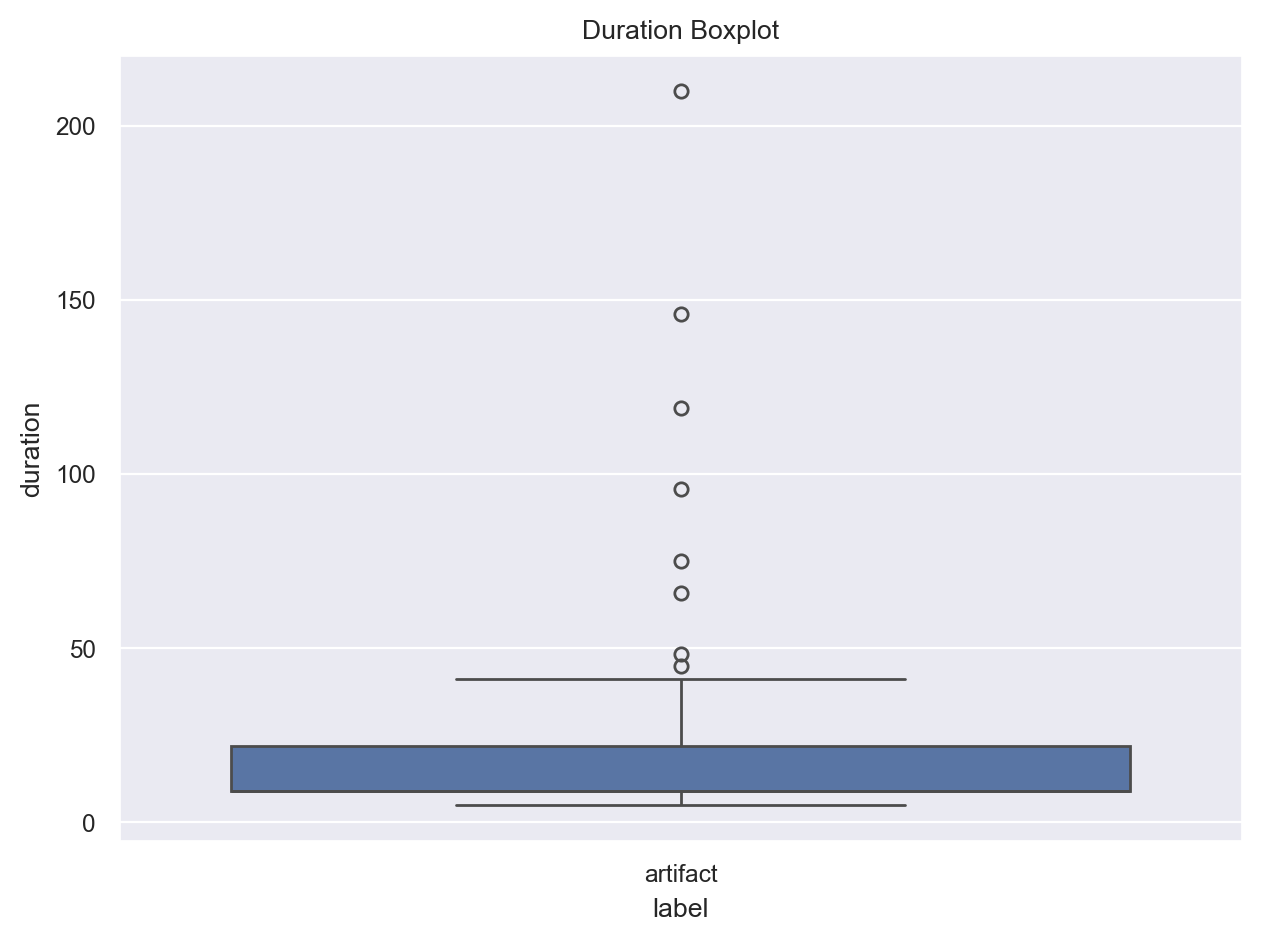
\includegraphics[width=1\columnwidth]{./images/DataExp_outliers_artifact.png}
	\caption{Outliers in the Artifacts class.}
	\label{fig:DataExp_outliers_Artifacts}
 \end{figure}